\documentclass[times,10pt,twocolumn]{article}
\usepackage{ipdps}
\usepackage{vmargin}
\setpapersize{USletter}
\setmargnohf{0.8125in}{1in}{6.875in}{8.875in}
\pagestyle{empty}
\newenvironment{twoaffiliations}{\begin{tabular}{cc}}{\end{tabular}}
\newenvironment{oddaffiliation}{\begin{center}}{\\~\\\end{center}}
%\documentclass[times,11pt,onecolumn]{article} 
%\usepackage{latex8}
%\usepackage{times}
\usepackage{epsfig}
%\pagestyle{empty}
%\newcommand{\mt}[1]{\mbox{#1}}

\title{MPEG-2 Decoding in a Stream Programming Language}

\author{
  Matthew Drake, Hank Hoffmann, Rodric Rabbah, and Saman Amarasinghe\\
  \begin{twoaffiliations}
    Massachusetts Institute of Technology\\
    Computer Science and Artificial Intelligence Laboratory\\
    \{madrake, hank, rabbah, saman\}@mit.edu
  \end{twoaffiliations}
}

\begin{document}
  
  \maketitle
  \thispagestyle{empty}
  
  \begin{abstract}
    Due to the high data rates involved in audio, video, and signal
processing applications, it is imperative to compress the data to
decrease the amount of storage used.  Unfortunately, this implies that
any program operating on the data needs to be wrapped by a
decompression and re-compression stage.  Re-compression can incur
significant computational overhead, while decompression swamps the
application with the original volume of data.

In this paper, we present a program transformation that greatly
accelerates the processing of compressible data.  Given a program that
operates on uncompressed data, we output an equivalent program that
operates directly on the compressed format.  Our transformation
applies to stream programs, a restricted but useful class of
applications with regular communication and computation patterns.  Our
formulation is based on LZ77, a lossless compression algorithm
utilized by ZIP, and immediately applies to simpler formats such as
Apple Animation, Microsoft RLE, and Targa.

We implemented a simple subset of our techniques in the StreamIt
compiler, which emits executable plugins for two popular video editing
tools: MEncoder and Blender.  For common operations such as color
adjustment and video compositing, computing directly on compressed
data offers a speedup roughly proportional to the overall compression
ratio.  For our benchmark suite of 12 videos in Apple Animation
format, speedups range from 1.1x to 471x, with a median of 15x.

  \end{abstract}
  
  \section{Introduction}


Stream computing represents an increasingly important class of
applications. In streaming codes, there is an abundance of parallelism that
is easier to extract compared to traditional desktop workloads (e.g.,
pointer-based computing). As a result, the extraction of parallelism
in streaming codes does not require heroic efforts, and thus,
processors can deliver higher performance with significantly lower
power costs. This is especially important since
leading microprocessor companies have realized that modern general
purpose architectures are near their  performance limits for  the
amount of power they consume. Thus, the future will place a greater
emphasis on exploiting the properties of streaming workloads in
conventional von~Neumann architectures.

Streaming is a model of computation that uses sequences of data
and computation kernels to expose concurrency and locality for
efficiency~\cite{wss}. In general purpose processors, improving locality 
translates to an effective management of the memory hierarchy at all
levels, including the register file. In this paper, we present a
methodology for compiling streaming codes to general purpose,
cache-based architectures. We first introduce a simple model for
reasoning effectively about the caching behavior of streaming
workloads. This model serves as a foundation for several {\it cache-aware
optimizations} that are geared toward the concomitant increase of instruction
and data {\it temporal locality}. These
optimization lead to significantly better utilization of the memory
system, and as such, they deliver performance gains ranging from 11
to 99\% for our streaming benchmark suite.

The context for our work is StreamIt, an architecture-independent
language that is engineered for streaming
applications~\cite{streamitcc}. It adopts the 
Cyclo-Static Dataflow~\cite{BELP96} model of computation which is a
generalization of Synchronous Dataflow~\cite{LM87-i} (SDF).  
SDF is a popular  model that  is well suited for
streaming codes. In SDF, computation is represented as a graph
consisting of {\it  actors} connected by communication channels; the
actors consume  and produce a constant number  of items from their
input and output  channels every time they execute. SDF is appealing
because it is amenable to static scheduling and optimization. 

From a general purpose architecture's point of view, actors represent
computation kernels, and the communication between actors represents
data buffers that must be streamed to and from the processor. Thus
the size of an actor and the
order of actor executions are critical properties that
impact the performance of the instruction cache. For example, the
compiler must make sure the actor's code size is not
greater than the instruction cache. Furthermore, we must {\it scale}
the execution of the actor so that it runs several times before we move
on to some other actor in the stream 
graph. This serves to $(i)$ amortize the cost of fetching the actor's
instructions into the cache from memory (an expensive operation), $(ii)$
improve the instruction temporal locality, and $(iii)$ improve overall
performance. However, as our cache model will show, we 
cannot arbitrarily scale the execution frequency of an actor. This
is because actors produce data that must be buffered, and therefore,
we must also consider the amount of data an actor produces and
consumes if we are to adequately manage the data cache. This paper is unique
in that it is the first to present a unified optimization methodology
that simultaneously considers instruction and data locality for
mapping streaming computation to cache-based architectures.

In terms of improving the data cache behavior, the compiler schedules
actor firing such that the producer-consumer locality is
preserved. Furthermore,  the compiler may {\it fuse}
together two or more actors to form a coarser grained kernel.
The fusion allows for better register allocation as we can
destroy the arrays used to buffer data between the actors and replace
the corresponding array references with scalars.  It also allows for
various competing implementations for managing the buffers between the
fused actors.  This paper evaluates several implementation
alternatives (for buffer management) and evaluates their performance.

The methodology for fusing actors leverages a distinguishing StreamIt
characteristic, namely, the hierarchical organization of
the stream graph. Furthermore, the algorithm for fusing actors applies
for the various topologies allowed by StreamIt.
It also considers another distinguishing characteristics of StreamIt,
namely the {\tt peek} operation whereby an actor may inspect data
items in its input buffer without consuming them until some future
execution. While peeking is a powerful language feature, it does pose
some challenges to the compiler and the cache optimizations. Peeking
also impacts the choice for the best buffer management strategy, as our
study will show.

%% the comment about p3 and itanium not being embedded architectures
%% is out of the blue! need a better transition.
Cache-aware fusion alone delivers significant performance gains, although our
evaluation shows that fusion with scaling leads to the best
performance on a general purpose, cache-based architecture. For our
experiments, we use two different processors: a superscalar out-of-order
processor, and an in-order VLIW processor. The former is a Pentium~3
whereas the latter is an Itanium~2. While these architectures are not
particularly suited for an embedded system, they do exhibit some
properties that are worthy of investigation. Furthermore, that we can
demonstrate measurable performance gains on real systems is far more
convincing than using a simulation-based environment. We chose the
Pentium~3 processor because it has very few registers in its
instruction set architecture. The Itanium by contrast has a much 
larger and richer repertoire of registers. The two architectures serve
to validate our cache-aware optimizations, in that we expect an
architecture with more register to benefit more from optimization such
as scalar replacement. On average, fusion leads to a 47\% improvement
on the Pentium~3, and 50\% on the Itanium~2.

The two architectures also differ in terms of their memory system
organization. The Itanium is an in-order VLIW processor and does not
tolerate a memory stall as well as its out-of-order
counterpart. Therefore we expect different gains from the scaling
optimization which amortize the long access latencies for instruction
and data caches. On average, scaling leads to a 21\% improvement on
the Itanium~2, and 17\% on the Pentium~3.

While both scaling and fusion lead to modest performance gains, we
must combine the two to deliver the best possible performance. When we
do so, we can further improve the performance of our benchmarks by
53\% on average for the Pentium~3, and 55\% for the Itanium~2.

\subsection{Summary of Contributions}

This paper makes the following contributions:
\begin{itemize}

\item A cache model for stream computing that provides a quantitative
estimate of the caching performance for any sequence of actor
executions.

\item A cache-aware scheduling heuristic that judiciously increases
the multiplicity of actors, improving instruction and data locality
while not exceeding the data cache.

\item A cache-aware partitioning policy that judiciously fuses
adjacent actors into a single component, enabling local optimizations
while not exceeding the instruction cache.

\item An optimized buffer management policy, termed ``copy-shift with
execution scaling'', which out-performs a traditional rotating buffer
in a detailed micro-benchmark analysis.

\item A fully automatic implementation of the above techniques in the
StreamIt compiler.

\item An experimental evaluation across 11 streaming benchmarks,
demonstrating performance improvements of up to 99\%.
\end{itemize}

\subsection{Paper Roadmap}

The remainder of the paper is organized as follows. Section~\ref{sec:streamit}
describes StreamIt and introduces our motivating example.
Section~\ref{sec:cache-model} introduces our cache model for 
reasoning about the performance of a streaming
computation. Section~\ref{sec:cache-opt} describes our cache-aware
optimizations, and Section~\ref{sec:buffer} describes the 
optimization enabled by fusion. Section~\ref{sec:evaluation} describes
our evaluation methodology and present our experimental
analysis. Sections~\ref{sec:related-work}~and~\ref{sec:conclusion}
discuss related work and concludes the paper.

  \Section{MPEG-2 Video Coding and Decoding}

MPEG-2~\cite{MPEG2} is a popular coding and decoding standard
for digital video data. The scheme is a subset of both the
DVD-Video~\cite{DVDVideo} standard for storing movies, and the Digital
Video Broadcasting specifications for transmitting HDTV and
SDTV~\cite{DVB}. The scheme is used by a wide variety of multimedia
applications and appliances such as the Tivo Digital Video
Recorder~\cite{tivo}, and the DirecTV satellite broadcast
service~\cite{directv}.

MPEG-2 encoding uses both {\it lossy} compression and {\it lossless}
compression. Lossy compression permanently eliminates information from
a video based on a human perception model. Humans are much better at
discerning changes in color intensity (luminance information) than
changes in color (chrominance information). Humans are also much more
sensitive to low frequency image components, such as a blue sky, than
to high frequency image components, such as a plaid shirt. Details
which humans are likely to miss can be thrown away without affecting
the perceived video quality.

Lossless compression eliminates redundant information while allowing
for its later reconstruction. Similarities between adjacent video
pictures are encoded using motion prediction, and all data is Huffman
compressed\cite{Huffman52}. The amount of lossy and lossless
compression depends on the video data. Common compression ratios range
from 10:1 to 100:1. For example, HDTV with a resolution of 1280x720
pixels and a streaming rate of 59.94 frames per second, has an
uncompressed data rate of 1.33 Gigabits per second. It is compressed at 
an average rate of 66:1, reducing the required streaming rate to
20 Megabits per second~\cite{imagevidstandards, Page 3}.

\SubSection{MPEG Coding}

\begin{figure}[t]
\begin{center}
\vspace{-12pt}
% \framebox{
% \includegraphics[scale=1, angle=0]{./mpeg-encoder.eps}
%}
% \vspace{-6pt}
% \nocaptionrule
 \caption{MPEG encoder.}
 \label{fig:mpeg-encoder}
%\vspace{-18pt}
\end{center}
\end{figure}

An overview of the encoding process is illustrated in
Figure~\ref{fig:mpeg-encoder}. The encoder operates on a sequence of
pictures. Each picture is made up of pixels arranged in a 16x16 array
known as a macroblock. Macroblocks are formed from 8x8 arrays, 
known as blocks, which contain pixel data for a single color channel. 
Each color channel in a macroblock may be represented by a 2x2 matrix
of blocks, or downsampled to a 1x2 or 1x1 block representation.
The compression in MPEG is achieved largely via motion estimation, which
detects and eliminates similarities between macroblocks across
pictures. Specifically, the motion estimator calculates a motion
vector to represent the horizontal and vertical displacement of a
given macroblock (i.e., the one being encoded) to a matching
macroblock-sized area in a reference picture. 
The matching macroblock is removed (subtracted) from the
current picture on a pixel by pixel basis. The result is a residual
predictive-code (P) picture. It represents the difference between the
current picture and the reference picture. Reference pictures encoded without
the use of motion prediction are intra-coded (I) pictures. In addition to forward
motion prediction, it is possible to encode new pictures using motion
estimation from both previous and subsequent pictures. Such pictures
are bidirectionally predictive-coded (B) pictures, and they exploit a
greater amount of temporal locality.

Each of the I, P, and B pictures then undergoes a 2-dimensional
discrete cosine transform (DCT) which separates the picture into parts
with varying visual importance. The input to the DCT is one block. 
The output of the
DCT is an 8x8 matrix of frequency coefficients. The upper left corner
of the matrix represents low frequencies, whereas the lower right
corner represents higher frequencies. The latter are often small and
can be neglected without sacrificing human visual perception.

\begin{figure}[t]
\begin{center}
\vspace{-12pt}
% \framebox{
% \includegraphics[scale=1, angle=0]{./zigzag.eps}
%}
% \vspace{-6pt}
% \nocaptionrule
 \caption{Zig-Zag scan patterns.}
 \label{fig:zigzag}
%\vspace{-18pt}
\end{center}
\end{figure}

The DCT coeffecients are quantized to reduce the number of bits needed
to represent them. Following quantization, many coefficients are
effectively reduced to zero. The DCT matrix is then run-length
encoded by emitting each non-zero coefficient, followed by the number
of zeros that precede it, along with the number of bits needed to
represent the coefficient, and its value. The run-length encoder
scans the DCT matrix in a zig-zag order (Figure~\ref{fig:zigzag}) to
consolidate the zeros in the matrix.

Finally, the output of the run-length encoder, motion vector data,
and other information (e.g., type of picture), are Huffman coded to 
further reduce the average number of bits per data item. The compressed
stream is sent to the output device.

\SubSection{MPEG Decoding}

An MPEG-2 input stream is organized as a Group of Pictures (GOP)
which contains all the information needed to reconstruct a video. The
GOP contains the three kinds of pictures produced by the encoder,
namely I, P, and B pictures. I pictures are intended to assist scene
cuts, random access, fast forward, or fast reverse
playback~\cite{MPEG2, Page 14 6.1.1.7}. A typical I:P:B picture ratio
in a GOP is 1:3:8, and a typical picture pattern is a
repetition of the following sequence: I B B P B B P B B P B B. The
input pictures are not ordered temporally within the stream. Rather,
they are ordered such that if a decoder encounters a P picture, its
motion prediction is with respect to the previously decoded I or P
picture, and if the decoder encounters a B picture, its motion
prediction is with respect the previously two decoded I or P pictures.

As with the encoding process, pictures are divided up into 16x16 pixel
macroblocks, themselves composed of 8x8 blocks. Macroblocks
specify colors using a {\it luminance} channel to represent saturation
(color intensity), and two {\it chrominance} channels to represent
hue. MPEG-2 streams specify a chroma format which allows the
chrominance data to be sampled at a lower rate. The most common chroma 
format is 4:2:0 which represents a macroblock using four blocks for the
luminance channel and one block for each of the two chrominance
channels. 

\begin{figure}[t]
\begin{center}
\vspace{-12pt}
% \framebox{
% \includegraphics[scale=1, angle=0]{./mpeg-decoder.eps}
%}
% \vspace{-6pt}
% \nocaptionrule
 \caption{MPEG decoder.}
 \label{fig:mpeg-decoder}
%\vspace{-18pt}
\end{center}
\end{figure}

The decoding process is illustrated in
Figure~\ref{fig:mpeg-decoder}. It is conceptually the reverse of the
encoding process. The input stream is Huffman and run-length decoded,
resulting in quantized DCT matrices. The DCT coefficients are scaled
in magnitude and an inverse DCT (IDCT) maps the frequency matrices to
the spatial domain.

Finally, the motion vectors parsed from the data stream are passed to
a motion compensator, which reconstructs the orginal pictures. In the
case of I pictures, the compensator need not make any changes since
these pictures were not subject to motion estimation~\footnote{I 
pictures are allowed to contain concealment motion vectors which aid in
macroblock reconstruction should a bitstream error destroy the 
frequency coefficient data. We ignore this special case.}. In the case of P
and B pictures however, motion vectors are used to find the
corresponding region in the current reference pictures. The
compensator then adds the relevant reference macroblocks to the
current picture to reconstruct it. These pictures are then emitted to
an output device.
  \section{StreamIt}
\label{sec:streamit}

StreamIt  is   an  architecture-independent  language that was
designed for  streaming applications. In StreamIt, programs are
represented as graphs where  nodes represent  computation and edges
represent FIFO-ordered communication of data over tapes.

The  basic programmable  unit (i.e., an actor) in  StreamIt is a {\it
filter}.   Each filter contains  a work  function that executes
atomically,  popping (i.e., reading)  a fixed number  of items  from
the  filter's input  tape and pushing (i.e., writing) a fixed number
of items to the filter's output tape.  A filter  may also {\tt peek} at
a given index  on its input tape without  consuming  the  item;  this
makes  it  simple  to  represent computation over a
sliding-window.   The {\tt push}, {\tt pop}, and {\tt peek} rates are
declared as part  of  the work  function,  thereby enabling  the
compiler    to construct a static schedule of filter executions. The
following is an example implementation of a FIR   (Finite Impulse
Response)  filter: 
%\begin{scriptsize}
{\small
\begin{verbatim}
float->float filter FIR (int N, float[] weights) 
{
  work push 1 pop 1 peek N {
    float sum = 0;
    for (int i = 0; i < N; i++) {
      sum += peek(i) * weights[i];
    }
    pop();
    push(sum);
  }
}
\end{verbatim}}
%\end{scriptsize}

The work function is invoked (fired) whenever there is sufficient data
on the input tape. In this case, the filter requires at least
\texttt{N} elements before it can execute. The value of \texttt{N} is
known at compile time when the filter is composed to form a stream
graph. A filter is akin to a class in object oriented programming
with the work function serving as the main method. The parameters
to a filter (e.g., \texttt{N} and \texttt{weights}) are equivalent to
parameters passed to a class constructor. In StreamIt, the
application developer focuses on the hierarchical assembly of the
stream graph and its communication topology, rather than on the 
explicit management of the data buffers between filters.

\begin{figure}[t]
\begin{center}
\vspace{-24pt}
 \framebox{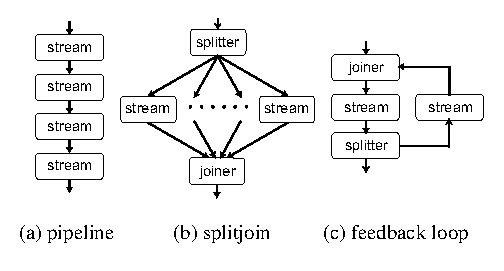
\includegraphics[scale=1, angle=0]{./constructs-eg.eps}}
 \vspace{-6pt}
 \caption{StreamIt containers.}
 \label{fig:containers}
\end{center}
\end{figure}

\begin{figure}[t]
\begin{center}
\vspace{-12pt}
 \framebox{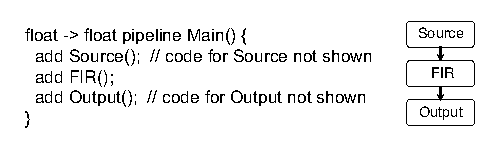
\includegraphics[scale=1, angle=0]{./pipeline-eg.eps}}
 \vspace{-6pt}
 \caption{Example pipeline with FIR filter.}
 \label{fig:pipeline}
\vspace{-18pt}
\end{center}
\end{figure}

StreamIt provides three hierarchical structures for composing filters
into larger stream graphs (see Figure~\ref{fig:containers}). The 
{\it pipeline} construct composes streams in sequence, with the output
of one connected to the input of the next.   An example of a pipeline
appears in Figure~\ref{fig:pipeline}.

The {\it splitjoin} construct distributes data to a set of parallel
streams, which are then joined together in a round robin fashion.  In
a splitjoin, the {\it splitter} performs the data scattering, and the
{\it joiner} performs the gathering. A splitter is a specialized
filter with a single input and  multiple output channels. On 
every execution step, it can distribute its output to any one of
its children in either a {\it duplicate} or a {\it roundrobin}
manner. For the former, incoming data is replicated to every
sibling connected to the splitter. For the latter, data is scattered
in a round-robin manner, with each item sent to exactly one child
stream, in order.  The splitter type and the weights for distributing data to
child streams are declared as part of the syntax (e.g., \texttt{split
duplicate} or \texttt{split roundrobin($w_0$, $w_1$, ... $w_n$)}). The
splitter counterpart, the joiner, is a specialized filter with  
multiple input channels but only one output channel. The joiner
gathers data from its predecessors in a round-robin manner (declared
as part of the syntax). 

StreamIt also provides a {\it feedback loop} construct for introducing
cycles in the graph.

\section{Execution Model}
\label{sec:execmodel}

A StreamIt program is represented by a hierarchical graph,
where the leaf nodes are filters, splitters, and joiners, and
the composite nodes are pipelines, splitjoins, and
feedback-loops. Edges in the graph represent data channels, which 
operate as FIFO queues.
In order for an actor  (i.e., a filter,
splitter, or joiner) to execute, it must have enough data items on its input
tape. In StreamIt, actors have  two epochs
of execution: one for initialization, and one for the steady
state. The initialization primes the input tapes to allow filters with
peeking to execute the very first instance of their work functions;
initialization in this setting is similar to the prologue stage in
software pipelining. The steady state schedule has the property that
the amount of data buffered between any two actors does not change
before and after the actor executions.

\begin{figure}[t]
\begin{center}
\vspace{-24pt}
 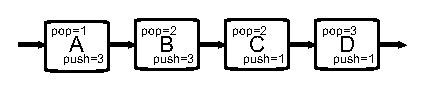
\includegraphics[scale=1, angle=0]{./pipe-with-rates.eps}
\vspace{-6pt}
 \caption{Example pipeline.}
 \label{fig:pipe-with-rates}
\end{center}
\end{figure}

As an example, a steady state schedule for the sample pipeline in
Figure~\ref{fig:pipe-with-rates} requires filter \texttt{A} to fire
four times, \texttt{B} six times, \texttt{C} nine times, and
\texttt{D} three times. 
% Because in StreamIt the filters are
% independent (i.e., they do not share state), they can execute
% concurently. In a uniprocessor setting (which is what we use for our
% evaluation), we can only run one filter at time. Therefore, 
The data generated by one actor is buffered (cached) until it is
consumed.

The StreamIt compiler derives the initialization and steady state
schedules~\cite{karczma-lctes03} and outputs a C program that includes
the initialization and work functions, as well as a driver to execute
each of the two schedules. For example, referring to
Figure~\ref{fig:pipe-with-rates}, the compiler generates the following
sample code for running the steady state schedule:
%\begin{scriptsize}
\begin{verbatim}
run_steady_state() {
  for (i = 0; i < 4; i++) A_work();
  for (i = 0; i < 6; i++) B_work();
  for (i = 0; i < 9; i++) C_work();
  for (i = 0; i < 3; i++) D_work();
}
\end{verbatim}
%\end{scriptsize}
To execute the program, the steady state kernel is wrapped with
another loop that invokes the kernel a designated number of
times. Preceding the state steady, a similar initialization schedule
is run to prime the data buffers, and following the steady state, an
epilogue is run to drain the buffers as necessary.

\begin{figure}[t]
\begin{center}
\vspace{-12pt}
 \psfig{figure=ssi.eps,width=3in}
 \vspace{-6pt}
 \caption{Instruction size (in bytes along the y-axis) per filter
 (x-axis) occurring in a steady state execution of FFT.}
 \label{fig:ssi-single}
\vspace{-18pt}
\end{center}
\end{figure}

From a caching point of view, it is intuitively clear that once a
filter's instruction working set is fetched into the cache, we must
execute that filter as many times as possible to improve instruction
locality and amortize the cost of the accesses to lower levels of the
memory hierarchy. This of course assumes that the total code size for
the filters in the steady state exceeds the capacity of the
instruction cache (which is commonly the case;). In
Figure~\ref{fig:ssi-single} we show a representative breakdown of the
code size per filter in a steady state execution of a StreamIt
implementation of FFT. In all, the total code size for a steady state
ranges from 16~Kb to over 60~Kb for our benchmarks. These results
provide evidence that while individual filters may have a
small instruction footprint, the total footprint of the filters in a
steady state exceeds a typical instruction cache size.
From these observations, it is evident that we must {\it scale} the
execution of filters in the steady state in order to improve temporal
locality. In other words, rather than running a filter $S$ times per
steady state, we increase the loop bound so that it runs $\texttt{M}
\times S$ times (e.g., the loop bound for \verb+A_work+ is
changed to $\texttt{M} \times 4$ in the example shown earlier). 
We term \texttt{M} the {\it multiplicity factor}.

The obvious question is: to what extent can we scale the execution of
filters in the steady state? The answer is non-trivial because
scaling, while beneficial to the instruction cache behavior, may
overburden the data cache as the buffers between actors may grow to
prohibitively large sizes that degrade the data cache
behavior. Specifically, if a buffer overflows the cache, then
produce-consumer locality is lost. 

Also complicating matters is the amount of state a filter must retain
from one execution of its work function to the next. In the FIR
example shown earlier, the filter state is proportional to the size of
the coefficient array (i.e., \texttt{weights}). The filter state
further constrains the schedule scaling.

  \Section{MPEG Decoder in StreamIt}

% TODO: recalculate lines of code using statement count (num of ;)
We implemented an MPEG-2 decoder in StreamIt. It is a fully portable
implementation in that the application is not architecture
dependent. The implementation was carried out by one student
programmer with no prior understanding of MPEG. The development
spanned eight weeks from specification~\cite{MPEG2} to the first fully
functional MPEG decoder. The StreamIt code is nearly 4,921 lines of
code with 48 static streams. The MPEG stream parser is the largest
single filter, consisting of 1,924 lines of code.  The 48 static
streams are compiled to 2,150 filters for a picture resolution of
352x240. In contrast, the reference C
implementation~\cite{reference-mpeg-c} is nearly 9,832 lines of code,
although it provides several features such as interlacing and
multi-layer streams that are not yet implemented in the StreamIt
decoder.

A noteworthy aspect of the StreamIt implementation is its
malleability. We illustrate this using two specific examples.  In the
first example, we focus on the video sampling rates. MPEG-2 streams
are encoded using a 4:2:0 sampling rate, which achieves a 50\%
reduction in the number of bits required to represent a video, with
little noticeable loss of color information. However, better quality
is possible with higher sampling rates since more color information is
retained from the original picture. In this paper, we describe how our
decoder implementation, originally designed to deal with a 4:2:0
sampling rate is modified for a 4:2:2 sampling rate.

In the second example, we describe a straight forward language-level
transformation that exposes the data-parallelism across macroblocks in
a picture. This is done in the context of the decoder pipeline which
consists of the inverse quantization, inverse DCT, and motion
compensator. We show that parallelism can be exposed at various levels
in the decoding process, from macroblock to block granularities, and
that the migration path is trivial.

\Section{Code Malleability: A Case Study}
\label{section:chroma}

To illustrate the concrete benefits of programming in a stream
language, we compare the support for varying chroma formats in the
StreamIt and C implementations.  While the conceptual difference
between chroma formats is merely a change in downsampling ratio, this
leads to a change in the data rates and the ratios of data between the
color channels. This requires that the C implementation parameterize
its buffer sizes, array lengths, array indices, and pointer offsets on
the chroma format; the reference implementation uses a ``chroma flag''
to dictate control flow to alternate index/offset calculations in 43
locations in the code. As an example, a fragment of the
``form\_prediction'' routine (in recon.c~\cite{reference-mpeg-c}) used
for motion compensation is shown in Figure~\ref{fig:chroma}. This
function calls a subroutine to perform the actual motion compensation
on each of the three color channels, passing in array offsets to a
global array holding the data. Lines 4-6 adjusts values used for
address calculations to handle the 4:2:2 and 4:2:0 chroma formats, and
lines 7-9 provide additional adjustments for the 4:2:0 format. While
these offset adjustments are necessary in C, they are difficult for
programmers and make the code hard to understand.

To add support for the 4:2:2 chroma format in our StreamIt decoder, we
modified 31 lines and added 20 new lines. Of the 31 modified lines, 23
were trivial modifications to pass a variable representing the chroma
format as a stream parameter. The greatest substantial change was to
the color channel splitter, previously illustrated on line 20 of
Figure~\ref{fig:dec0with-code}. In the case of a 4:2:2 sampling
rate, the chrominance data, as it appears on the input tape,
alternates between each of the two chrominance channels. Thus, a
nested splitjoin is used to properly recover the appropriate
chrominance channels. The new splitjoin is shown in
Figure~\ref{fig:chroma}.  Even after these modifications, the chroma
format only explicitly dictates control flow in 9 locations. Of
course, the scheduling and buffer management changes dramatically
between chroma formats, but this is automatic and hidden from the
programmer.

\begin{figure*}[t]
 \begin{minipage}[t]{4.3in}
   {
   % Matt's note - this is the C reference code I added.
   % I added the line numbers so I can reference them in the text.
    \begin{scriptsize}
    \begin{verbatim}
1    /* Y */
2    form_component_prediction(src[0]+(sfield?lx2>>1:0),dst[0]+(dfield?lx2>>1:0),
3                              lx,lx2,w,h,x,y,dx,dy,average_flag);
4    if (chroma_format!=CHROMA444)  {
5        lx>>=1; lx2>>=1; w>>=1; x>>=1; dx/=2;
6    }
7    if (chroma_format==CHROMA420)  {
8        h>>=1; y>>=1; dy/=2;
9    }
10   /* Cb */
11   form_component_prediction(src[1]+(sfield?lx2>>1:0),dst[1]+(dfield?lx2>>1:0),
12                             lx,lx2,w,h,x,y,dx,dy,average_flag);
13   /* Cr */
14   form_component_prediction(src[2]+(sfield?lx2>>1:0),dst[2]+(dfield?lx2>>1:0),
15                             lx,lx2,w,h,x,y,dx,dy,average_flag);    
    \end{verbatim}
    \end{scriptsize}
   }
   % \vspace{-3pt}
   % \caption{Decoding stream to handle 4:2:0 and 4:2:2 chroma formats.}
   % \label{fig:chroma-stream}
  \end{minipage}
    ~~\hrule~~
 \begin{minipage}[t]{4.3in}
   {
    \begin{scriptsize}
    \begin{verbatim}
    // C = blocks per chrominance channel per macroblock 
    // C = 1 for 4:2:0, C = 2 for 4:2:2
    add splitjoin {
      split roundrobin(4*(B+V), 2*C*(B+V));
      add MotionCompensation() to PT1;
      add splitjoin {
        split roundrobin(N, N);
        for (int i = 0; i < 2; i++) {
          add MotionCompensation() to PT1;
          add ChannelUpsample(C);
        }
        join roundrobin(1, 1);
      }
      join roundrobin(1, 1, 1);
    }
    \end{verbatim}
    \end{scriptsize}
   }
   % \vspace{-3pt}
   % \caption{Decoding stream to handle 4:2:0 and 4:2:2 chroma formats.}
   % \label{fig:chroma-stream}
  \end{minipage}
  ~~\vrule~~
  \begin{minipage}[t]{2.0in}
  {
   \begin{center}
    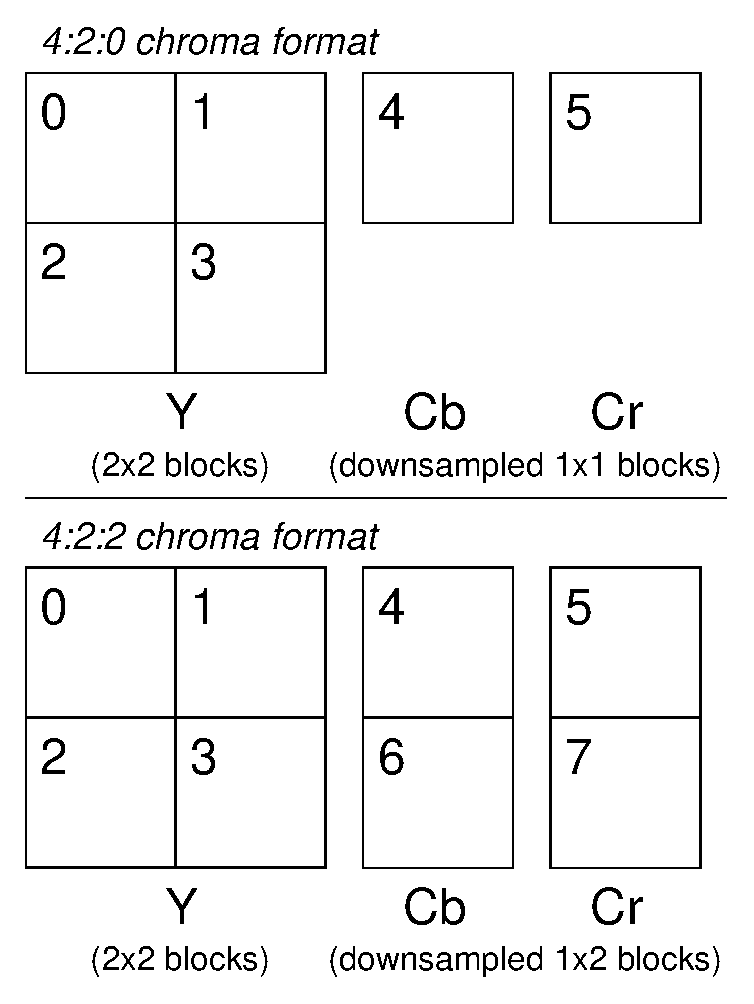
\epsfig{file=chroma_format.eps, width=2.5in}
    % \caption{4:2:0 and 4:2:2 chroma formats showing macroblock ordering}
    % \label{fig:chroma-format}
   \end{center}
  }
  \end{minipage}
  \caption{Decoding stream to handle 4:2:0 and 4:2:2 chroma
    formats. Figures on right illustrate how macroblock orderings
    differ.}
  \label{fig:chroma}
\end{figure*}

\SubSection{Motion Compensation}

An MPEG decoder accepts a bitstream as input and performs Huffman and
variable run-length decoding (VLD).  This process results in a set of
quantized, frequency-domain macroblocks and corresponding motion
vectors.  The decoder inverse quantizes (IQ) the macroblocks and then
performs an inverse DCT (IDCT) to convert the macroblocks to the
spatial domain.  For predictively coded macroblocks (e.g., P and B
pictures), the decoder performs motion compensation (MC) using the
input motion vectors to find a corresponding macroblock in a
previously decoded, stored reference picture. This reference
macroblock is added to the current macroblock to recover the original
picture data. If the current macroblock is part of an I or P picture,
then the decoder stores it for future reference.
Figure~\ref{fig:dec_block} illustrates the decode sequence.

\begin{figure}[htbp]
\centerline{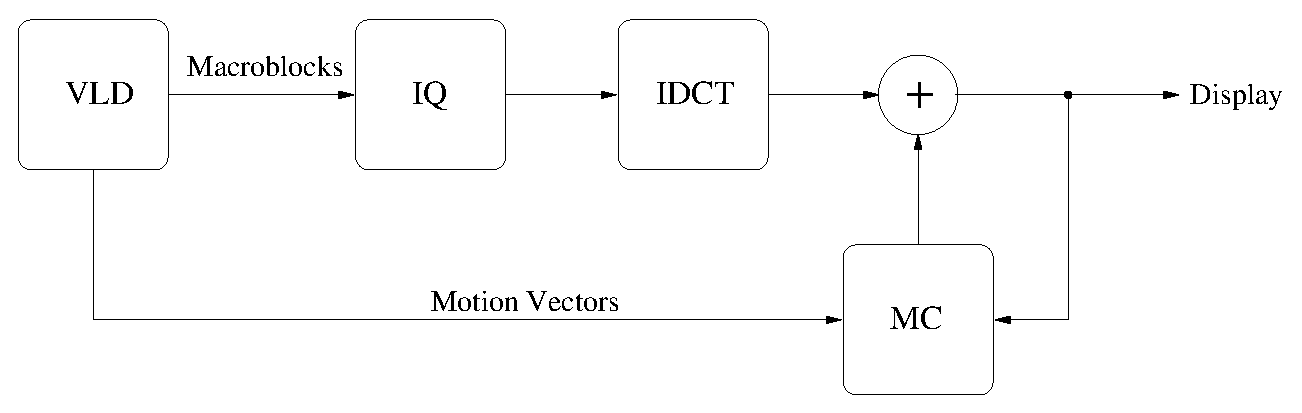
\epsfig{file=dec_block.eps,width=5in}}
\caption{Block diagram of MPEG-2 decode.}
\label{fig:dec_block}
\end{figure}

A simple strategy for parallelizing the MPEG-2 decoding can exploit
the data parallelism among macroblocks. Using this scheme, the Huffman
and run-length decoding is inherently serial, as macroblock boundaries
can only be discovered by performing the decode operation.  Once this
decode is complete, a parallel implementation can distribute
macroblocks to independent streams (using a splitjoin). Each stream
performs the inverse quantization, inverse discrete cosine transform,
and motion compensation. Furthermore, each stream locally stores
reference macroblocks for future motion compensation. Using this
strategy, the streams can execute independently with one exception.

% TODO: This is the figure showing the macroblock parallelism
% I'm not sure where it goes. - Matt
\begin{figure*}[t]
\vspace{-12pt}
%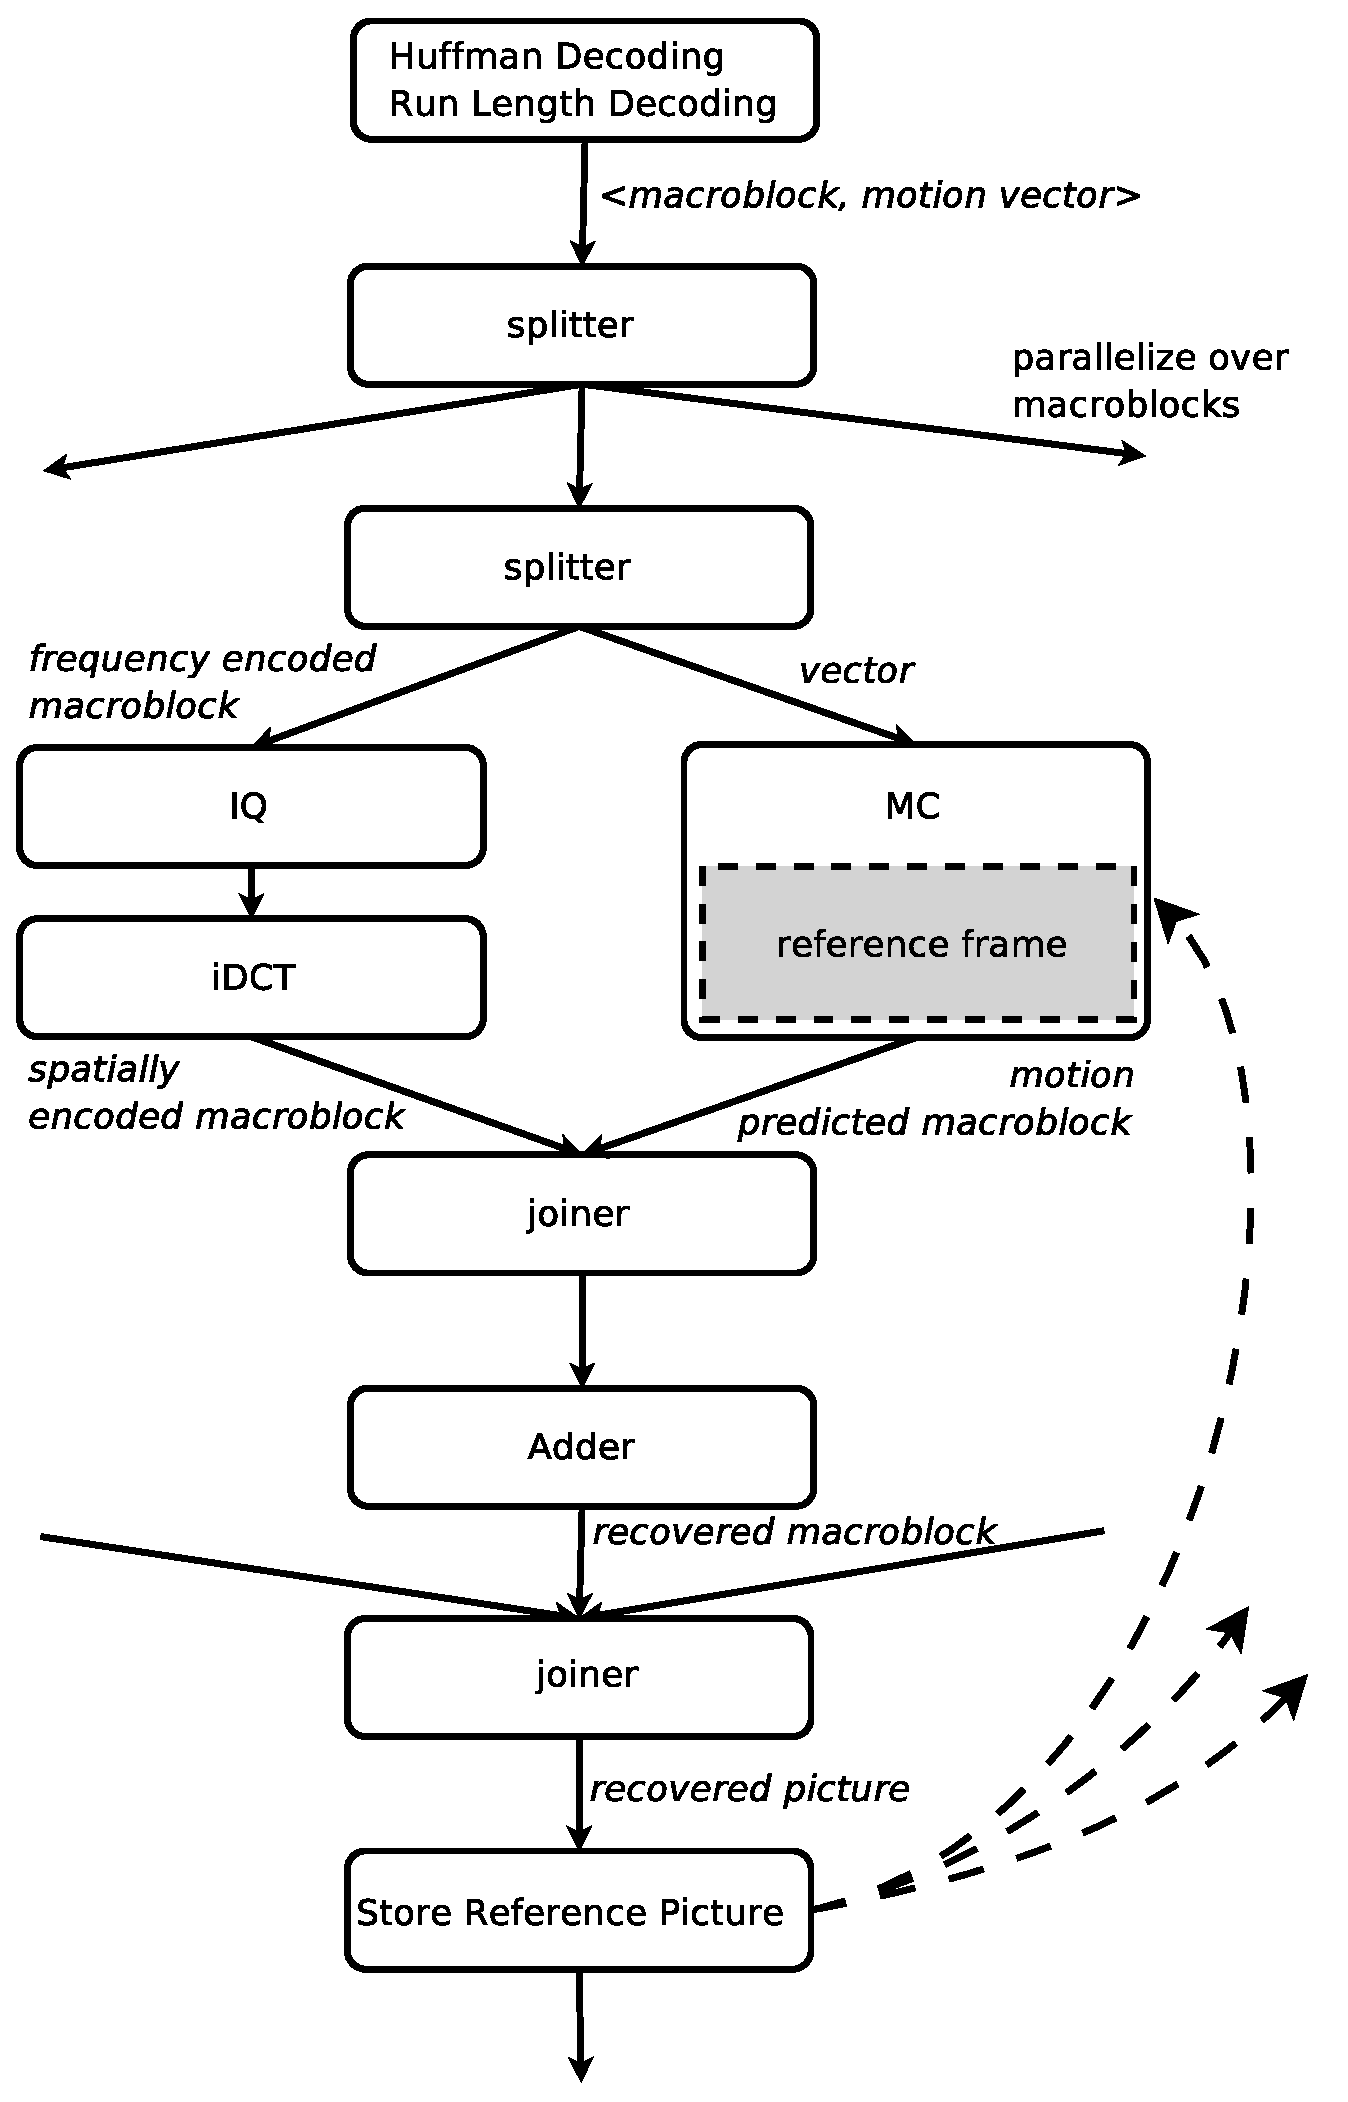
\epsfig{file=decoder_macroblock_parallelism.eps, width=3in}
%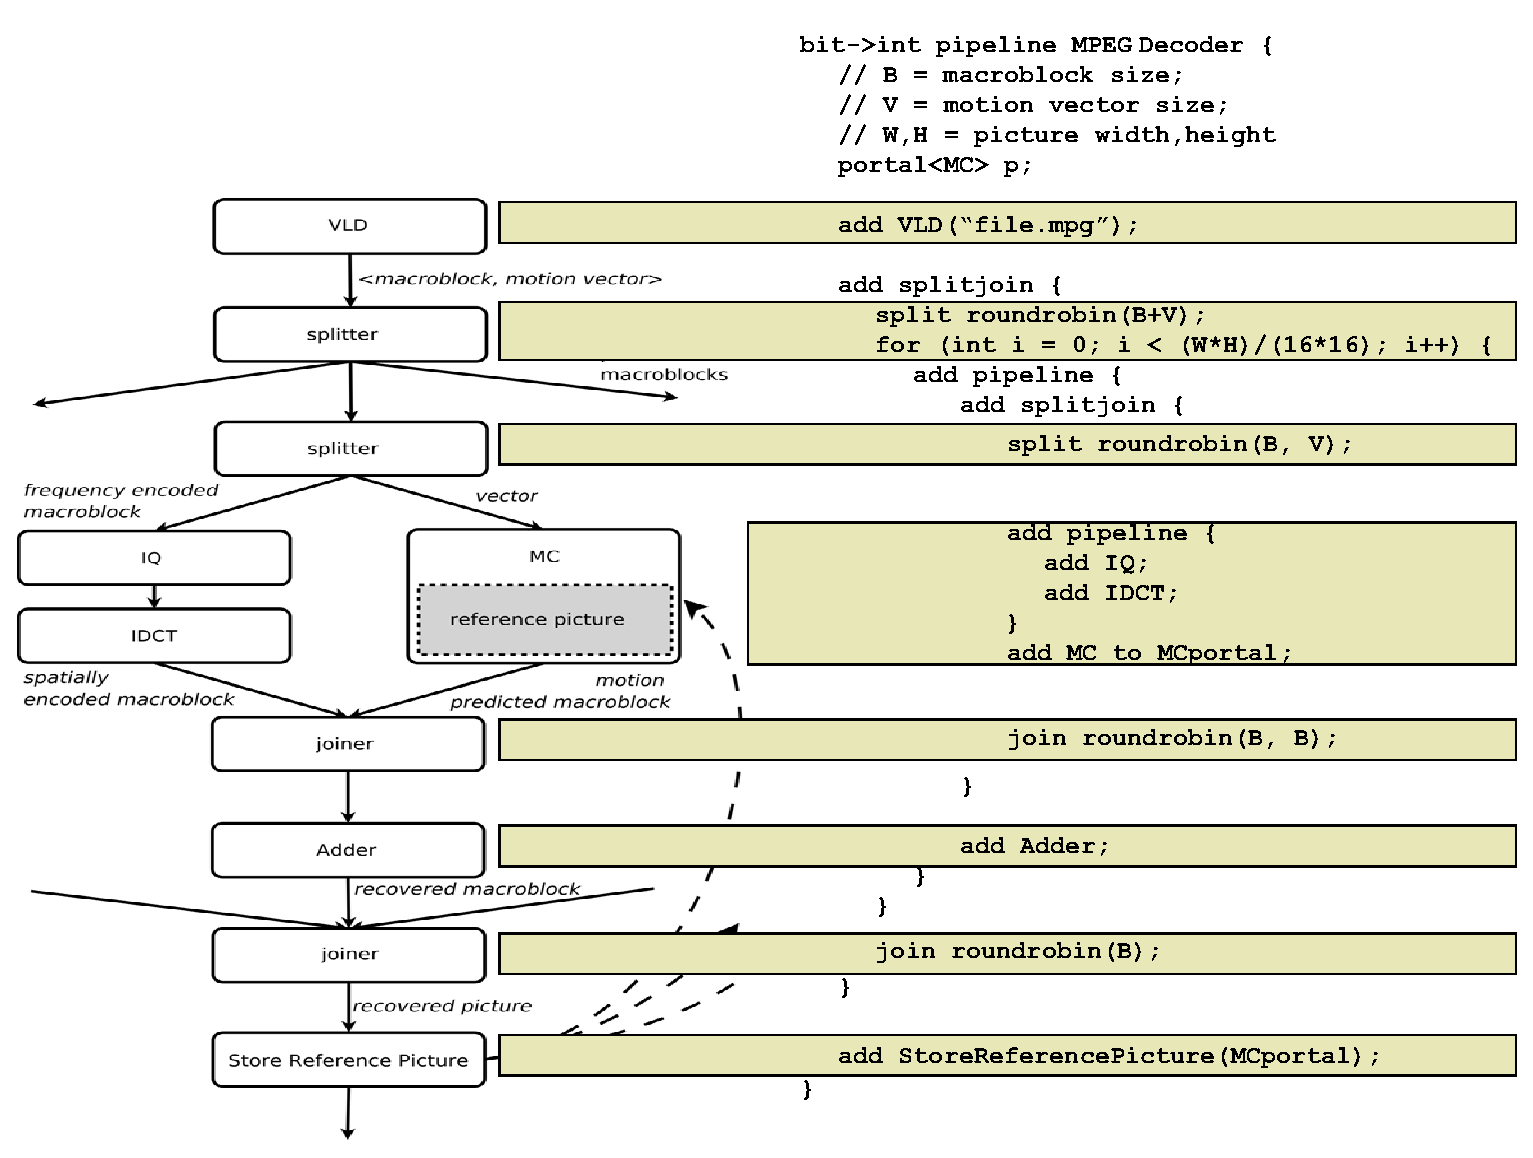
\epsfig{file=decoder-parallel.eps, width=\textwidth}
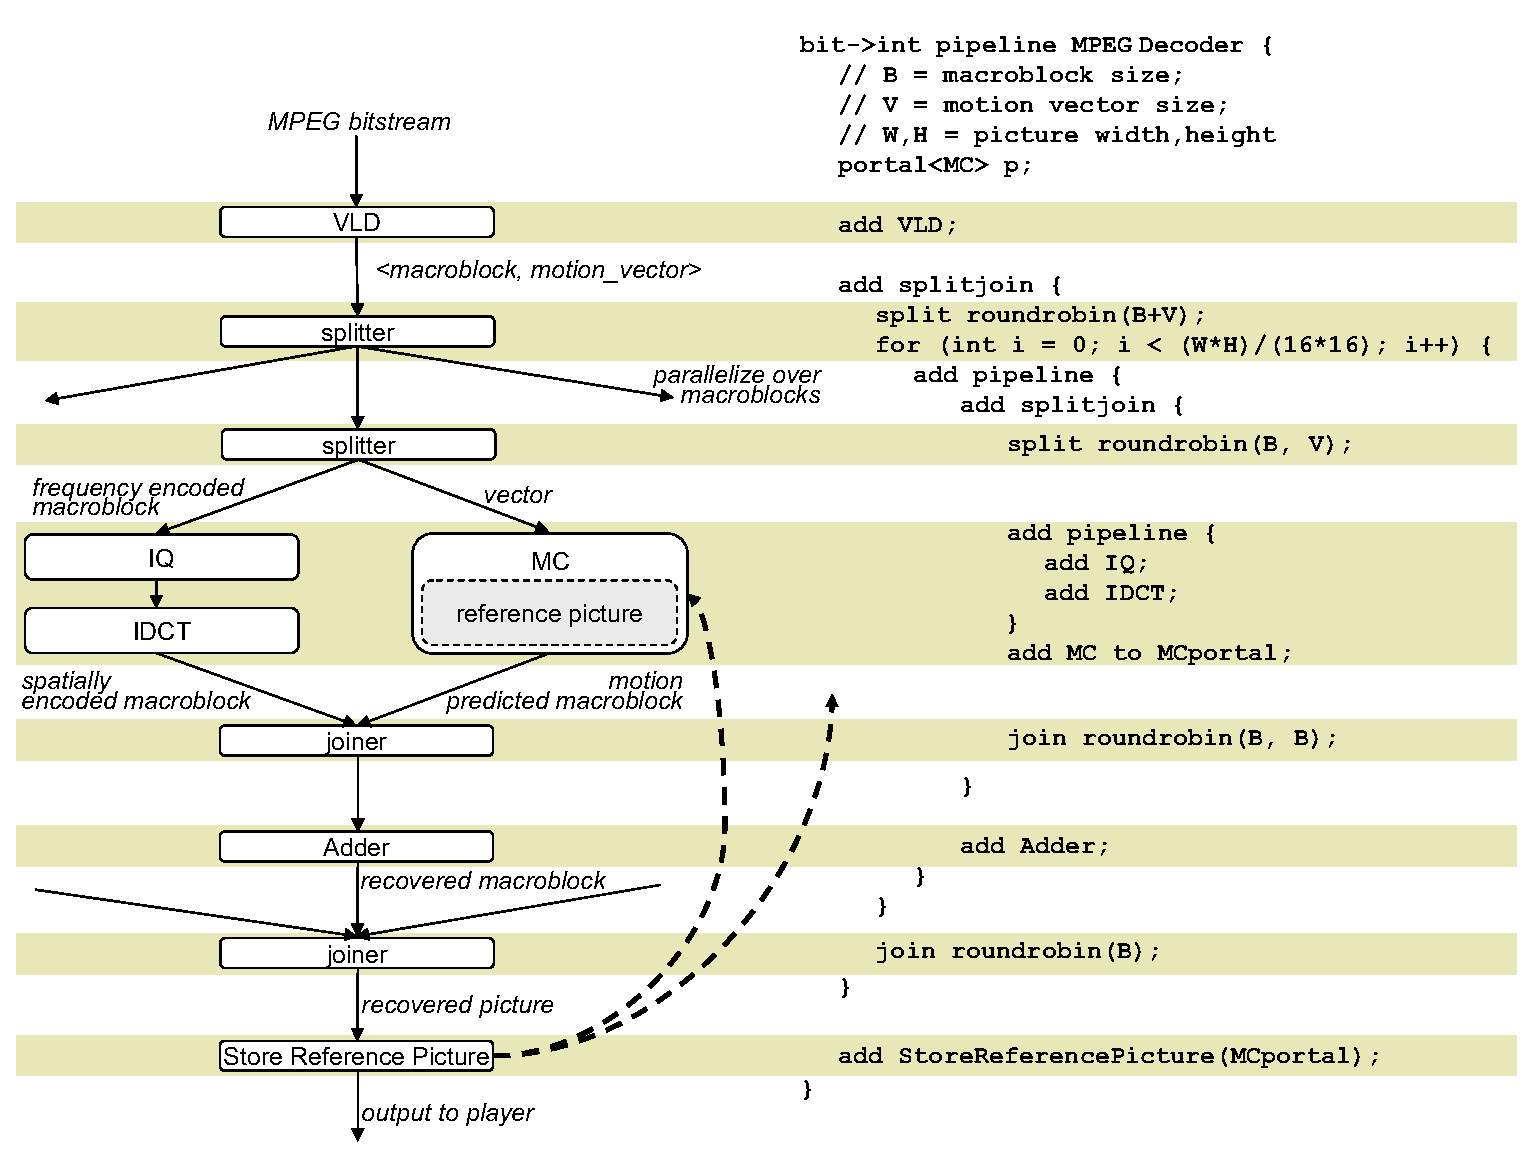
\epsfig{file=decoderpipeline.eps, width=\textwidth}
% TODO: Change Matt's 2 am caption.
\caption{MPEG-2 decoder exploiting macroblock-level parallelism.}
\label{decoder_macroblock_parallelism}
\vspace{-6pt}
\end{figure*}

This exception occurs when a stream is performing motion compensation
and the corresponding motion vector indicates a reference macroblock
stored in some other stream. In this case, inter-stream communication
is required to send the reference data to the requesting stream. This
situation is not uncommon, and is more prevalent for higher resolution
pictures. A simple scheme for handling this situation is for every
stream to broadcast its decoded macroblocks to all other streams. This
solution has the benefit of being conceptually easy to understand and
implement. StreamIt allows programmers to naturally expose such
parallelism. A StreamIt pipeline that operates at macroblock
granularity is shown in Figure~\ref{decoder_macroblock_parallelism}. It is
worthy to note that there is a high correlation between the stream
graph, and the StreamIt syntax describing the pipeline.

The implementation can be made more fine grained by exposing the
intra-macroblock parallelism. For example, the IQ-IDCT pipeline can
operate at a block level, rather than at a macroblock
granularity. This is easily achieved by encapsulating the IQ-DCT pipeline
within a splitjoin to scatter the blocks, operate, and gather the
results to recover the parent macroblock.

There are many implementation strategies for the decoder, each with
varying degrees of exposed parallelism. Of the greatest advantage of
the StreamIt implementation is its malleability. The stream graph is
easily reconfigured to operate at picture-level granularity (exposing
parallelism between chroma channels), macroblock level (exposing even
more data-level parallelism), or even at block level (exposing the
greatest amount of data-level parallelism). The modularity of the
language also affords the ability to cleanly define stream interfaces,
and reuse existing components. As an example, the zig-zag descrambler,
inverse quantizer, and inverse DCT components were all reused for our
JPEG codec implementation. The modularity also reduces the complexity
of the debugging process, as stream components can be functionally
verified independently, leading to greater programmer productivity.

%% TODO: add figure showing decoder pipeline at macroblock granularity
%% and streamit text ala Bill's beamformer/fmradio examples



  \Section{Code Malleability: A Case Study}
\label{section:chroma}

To illustrate the concrete benefits of programming in a stream
language, we compare the support for varying chroma formats in the
StreamIt and C implementations.  While the conceptual difference
between chroma formats is merely a change in downsampling ratio, this
leads to a change in the data rates and the ratios of data between the
color channels. This requires that the C implementation parameterize
its buffer sizes, array lengths, array indices, and pointer offsets on
the chroma format; the reference implementation uses a ``chroma flag''
to dictate control flow to alternate index/offset calculations in 43
locations in the code. As an example, a fragment of the
``form\_prediction'' routine (in recon.c~\cite{reference-mpeg-c}) used
for motion compensation is shown in Figure~\ref{fig:chroma}. This
function calls a subroutine to perform the actual motion compensation
on each of the three color channels, passing in array offsets to a
global array holding the data. Lines 4-6 adjusts values used for
address calculations to handle the 4:2:2 and 4:2:0 chroma formats, and
lines 7-9 provide additional adjustments for the 4:2:0 format. While
these offset adjustments are necessary in C, they are difficult for
programmers and make the code hard to understand.

To add support for the 4:2:2 chroma format in our StreamIt decoder, we
modified 31 lines and added 20 new lines. Of the 31 modified lines, 23
were trivial modifications to pass a variable representing the chroma
format as a stream parameter. The greatest substantial change was to
the color channel splitter, previously illustrated on line 20 of
Figure~\ref{fig:dec0with-code}. In the case of a 4:2:2 sampling
rate, the chrominance data, as it appears on the input tape,
alternates between each of the two chrominance channels. Thus, a
nested splitjoin is used to properly recover the appropriate
chrominance channels. The new splitjoin is shown in
Figure~\ref{fig:chroma}.  Even after these modifications, the chroma
format only explicitly dictates control flow in 9 locations. Of
course, the scheduling and buffer management changes dramatically
between chroma formats, but this is automatic and hidden from the
programmer.

\begin{figure*}[t]
 \begin{minipage}[t]{4.3in}
   {
   % Matt's note - this is the C reference code I added.
   % I added the line numbers so I can reference them in the text.
    \begin{scriptsize}
    \begin{verbatim}
1    /* Y */
2    form_component_prediction(src[0]+(sfield?lx2>>1:0),dst[0]+(dfield?lx2>>1:0),
3                              lx,lx2,w,h,x,y,dx,dy,average_flag);
4    if (chroma_format!=CHROMA444)  {
5        lx>>=1; lx2>>=1; w>>=1; x>>=1; dx/=2;
6    }
7    if (chroma_format==CHROMA420)  {
8        h>>=1; y>>=1; dy/=2;
9    }
10   /* Cb */
11   form_component_prediction(src[1]+(sfield?lx2>>1:0),dst[1]+(dfield?lx2>>1:0),
12                             lx,lx2,w,h,x,y,dx,dy,average_flag);
13   /* Cr */
14   form_component_prediction(src[2]+(sfield?lx2>>1:0),dst[2]+(dfield?lx2>>1:0),
15                             lx,lx2,w,h,x,y,dx,dy,average_flag);    
    \end{verbatim}
    \end{scriptsize}
   }
   % \vspace{-3pt}
   % \caption{Decoding stream to handle 4:2:0 and 4:2:2 chroma formats.}
   % \label{fig:chroma-stream}
  \end{minipage}
    ~~\hrule~~
 \begin{minipage}[t]{4.3in}
   {
    \begin{scriptsize}
    \begin{verbatim}
    // C = blocks per chrominance channel per macroblock 
    // C = 1 for 4:2:0, C = 2 for 4:2:2
    add splitjoin {
      split roundrobin(4*(B+V), 2*C*(B+V));
      add MotionCompensation() to PT1;
      add splitjoin {
        split roundrobin(N, N);
        for (int i = 0; i < 2; i++) {
          add MotionCompensation() to PT1;
          add ChannelUpsample(C);
        }
        join roundrobin(1, 1);
      }
      join roundrobin(1, 1, 1);
    }
    \end{verbatim}
    \end{scriptsize}
   }
   % \vspace{-3pt}
   % \caption{Decoding stream to handle 4:2:0 and 4:2:2 chroma formats.}
   % \label{fig:chroma-stream}
  \end{minipage}
  ~~\vrule~~
  \begin{minipage}[t]{2.0in}
  {
   \begin{center}
    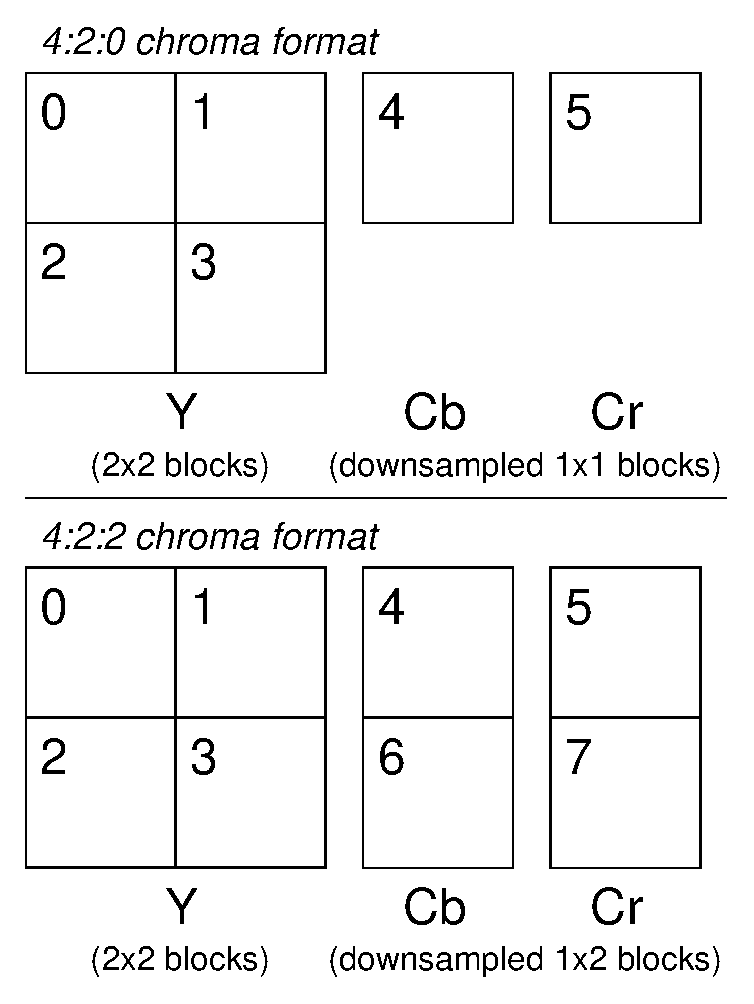
\epsfig{file=chroma_format.eps, width=2.5in}
    % \caption{4:2:0 and 4:2:2 chroma formats showing macroblock ordering}
    % \label{fig:chroma-format}
   \end{center}
  }
  \end{minipage}
  \caption{Decoding stream to handle 4:2:0 and 4:2:2 chroma
    formats. Figures on right illustrate how macroblock orderings
    differ.}
  \label{fig:chroma}
\end{figure*}
  %This section walks through a sample session with the compiler and
runtime system.  We will use the {\tt FMRadio} benchmark from the
StreamIt release as a running example.  To get started, change to the
following directory:
\begin{verbatim}
cd $STREAMIT_HOME/apps/benchmarks/fm/streamit
\end{verbatim}
The benchmark is in {\tt FMRadio.str}.  Note that it differs slightly
from the version developed in this cookbook.

\subsection{Compiling for a Uniprocessor}

To compile 


library
 ProgramName.dot

standalone

raw
rawcol
numbers
magic\_net (?)
simulatework
partition  (+greedy?)

linearpartition

standalone

-----

DOT FILES


  %\Section{MPEG Encoder in StreamIt}
  \section{Related Work}
\label{sec:related}

% BILL

%Signal~\cite{Signal}, 
%Lucid~\cite{Lucid77}, and
%Occam~\cite{Occam}, and Sisal \cite{sisal}.
%Parallel Haskell~\cite{ph}
In addition to StreamIt, there are a number of stream-oriented
languages drawing from domains such as functional, dataflow, CSP and
synchronous programming~\cite{survey97}.  The Brook language is
architecture-independent and focusses on data
parallelism~\cite{brook04}.  Stream kernels are required to be
stateless, though there is special support for reducing streams to a
single value.  Stream\-C/Ker\-nel\-C is lower level than Brook;
kernels written in KernelC are stiched together in StreamC and mapped
to the data-parallel Imagine processor~\cite{imagine03ieee}.  SPUR
adopts a similar decomposition between ``microcode'' stream kernels
and skeleton programs to expose data parallelism~\cite{spur05samos}.
Cg exploits pipeline parallelism and data parallelism, though the
programmer must write algorithms to exactly match the two pipeline
stages of a graphics processor~\cite{cg03}.  Compared to these
languages, StreamIt places more emphasis on exposing task and pipeline
parallelism (all the languages expose data parallelim).
%and on sliding window operations (filters that peek).  
By adopting the synchronous dataflow model of execution~\cite{lee87},
StreamIt focusses on well-structured programs that can be aggressively
optimized.  The implicit infinite loop around programs is also a key
StreamIt characteristic that enables the transformations in this
paper.  Spidle is also a recent stream language that was influenced by
StreamIt~\cite{spidle03}.
%and Lucid Synchrone~\cite{Lucid-Synchrone}.
%Synchronous languages which
%target embedded applications include Esterel~\cite{Esterel},
%Lustre~\cite{Lustre}, and Additional

Liao et al. map Brook to multicore processors by leveraging the affine
partitioning model~\cite{liao06brook}.  While affine partitioning is a
powerful model for parameterized loop-based programs, in StreamIt we
simplify the problem by fully resolving the program structure at
compile time.  This allows us to schedule a single steady state using
flexible, non-affine techniques (e.g., simulated annealing) and to
repeat the found schedule for an indefinite period at runtime.
Gummaraju and Rosenblum map stream programs to a general-purpose
hyperthreaded processor~\cite{gummaraju05micro}.  Such techniques
could be integrated with our spatial partitioning to optimize per-core
performance.  Gu et al. expose data and pipeline parallelism in a
Java-like language and use a compiler analysis to efficiently extract
coarse-grained filter boundaries~\cite{du03sc}.  Ottoni et al. also
extract decoupled threads from sequential code, using hardware-based
software pipelining to distribute the resulting threads across
cores~\cite{ottoni05decoupled}.  By embedding pipeline-parallel
filters in the programming model, we focus on the mapping step.

%%%%%%%%%%%%%%%%%%%%%%%%%%%%%%%%%%%%%%%%%%%%%%%%%%%%%%%%%%%%%%%%%%%%%

Previous work in scheduling computation graphs to parallel targets has
focused on partitioning and scheduling techniques that exploit task
and pipeline parallelism~\cite{SDFSched, SDFSched2,may87communicating,
DAGSched, pipeline-sdf}.  Application of loop-conscious
transformations to coarse-grained dataflow graphs has been
investigated.  Unrolling (or ``unfolding'' in this domain) is employed
for synchronous dataflow (SDF) graphs to reduce the initiation
interval but they do not evaluate mappings to actual
architectures~\cite{unfolding,unfolding2}. Software pipelining
techniques have been applied to SDF graphs onto various embedded and
DSP targets~\cite{bakshi99,chatha-02}, but has required programmer
knowledge of both the application and the architecture. To our
knowledge, none of these systems automatically exploit the combination
of task, data, and pipeline parallelism.  Furthermore, these systems
do not provide a robust end-to-end path for application
parallelization from a high-level, portable programming language.

%% Previous work on instruction-level software pipelining has focused
%% mostly on scheduling machine instructions in a loop via modulo
%% scheduling~\cite{rau81,lam-softpipe}.  The algorithms devised must
%% account for tight resource constraints and complex instruction
%% dependences. Our software-pipelining problem is much less constrained,
%% enabling us to employ a simple greedy heuristic.  

%% Furthermore, a traditional modulo scheduling algorithm is not needed
%% because we have an implicit loop barrier at the end of each
%% steady-state.  ILP compilers for clustered VLIW
%% architectures~\cite{Bulldog,Multiflow,lee98spacetime,qian02} must
%% partition instructions and assign them to clusters as part of the
%% instruction scheduling. Clustering is analogous to our application of
%% filter fusion in our software pipelining algorithm.

  %\Section{Concluding Remarks}
\vspace{-11pt}

As computer architectures change from the traditional monolithic
processors, to scalable wire-exposed and multicore processors, there
is a greater need for portable applications that expose parallelism
and communication to enable efficient and high performance
executions---while also boosting programmer productivity. StreamIt is
a programming language and a compilation infrastructure specifically
engineered to naturally expose and leverage stream abstractions that
are embodied in modern streaming applications. We have used StreamIt
to implement DSP codes (e.g., software radio, beamforming), image and
video codecs (e.g., MPEG-2 encoding and decoding), encryption
algorithms (e.g., DES and Serpent), and many other applications. The
language, compiler, and applications are available for download from
the project web page at http://cag.csail.mit.edu/streamit.

The goal of the StreamIt project is to boost productivity for
streaming application developers such that they focus on algorithmic
innovation rather than on performance tuning. The ability to leverage
domain specific language constructs affords optimization opportunities
that can deliver high performance from high levels of abstraction. 

We believe emerging languages such as X10 can provide a framework to
implement domain specific abstractions in a general purpose
programming model. We have designed and implemented a prototype bridge
to run StreamIt code as part of the X10 virtual machine. As a result,
application developers can use the streaming abstractions for the
computation that fit that model of computation, while different
abstractions can be used to describe other aspects of the computation.
A part of our ongoing work is concerned with evaluating the productivity
and performance merit of native interfaces to and from StreamIt codes.
  \section{Conclusion}
\label{sec:conclusion}

In this paper, we describe the StreamIt compiler for the Raw
architecture.  The stream graph of a StreamIt program exposes the data
communication pattern to the compiler while the lack of global
synchronization frees the compiler to radically reoganize the program
for efficient execution on the underline architecture. The StreamIt
compiler demonstrates the power of this flexibility by totally
reoganizing large programs for better load balance. We were able to
map many of programs on to the Raw processor and obtain good
performance.

We introduce a collection of optimizations, vertical and horizontal
filter fusion, vertical and horizontal filter fission and filter
reordering transformations, that can be used to restructure stream
graphs.  We show that by applying these transformations we can map a
high-level stream program, written to reflect the composition of the
application, onto Raw and achieve good processor utilization and load
balance, leading to a factor of three speedup on two applications.

Unlike all previous streaming languages, the structured streams of
StreamIt makes it possible for us to approach the optimization and
parallelization problems in a very systermatic manner. It enables us
to define multiple optimizations -- targetting different constructs
and requirements -- and to compose them them in a hirearchical manner.

The ability to do global transformations across multiple filters, that
may have originated from very different parts of the application,
makes it possible for the compiler to find optimization opportunities
that may ellude even an experience programmer.  Such capabilities
enables the programmers to write protable streaming applications and
map them efficiently onto any given architecture. This has the
potential of creating a programming standard for emerging
communication exposed architectures.  The StreamIt compiler takes a
fist step towards this goal.


  
  \vspace{-2pt}
  \section*{Acknowledgements}
  \vspace{-7pt}
  We are very grateful to the entire StreamIt team for their hard work
  and insightful comments. Allyn Dimock, Michael Gordon, Janis
  Sermulins, and especially William Thies, contributed immensely to
  the StreamIt infrastructure to enable this paper. We also thank the
  anonymous reviewers for their helpful suggestions. The StreamIt
  project is supported by DARPA grants PCA-F29601-03-2-0065 and
  HPCA/PERCS-W0133890, and NSF awards CNS-0305453 and EIA-0071841.

%  \bibliographystyle{ipdps}
%  \bibliography{main}
  \vspace{-2pt}
\begin{thebibliography}{10}\setlength{\itemsep}{-1ex}\small
  \vspace{-7pt}
\bibitem{agrawal05cases}
S.~Agrawal, W.~Thies, and S.~Amarasinghe.
\newblock Optimizing stream programs using linear state space analysis.
\newblock In {\em {CASES}}, 2005.

\bibitem{ahmad01multiproc}
I.~Ahmad, S.~M. Akramullah, M.~L. Liou, and M.~Kafeel.
\newblock {A Scalable Off-line MPEG-2 Video Encoding Scheme using a
  Multiprocessor System}.
\newblock {\em {Parallel Computing}}, 27, 2001.

\bibitem{ahmad01compression}
I.~Ahmad, Y.~He, and M.~L. Liou.
\newblock {Video compression with parallel processing}.
\newblock {\em {Parallel Computing}}, 28, 2002.

\bibitem{ph}
S.~Aidtya, Arvind, L.~Augustsson, J.~Maessen, and R.~S. Nikhil.
\newblock {Semantics of pH: A parallel dialect of Haskell}.
\newblock In {\em Haskell Workshop}, 1995.

\bibitem{Lucid77}
E.~Ashcroft and W.~Wadge.
\newblock Lucid, a non procedural language with iteration.
\newblock {\em C. ACM}, 20(7), 1977.

\bibitem{assayad05mpeg4b}
I.~Assayad, P.~Gerner, S.~Yovine, and V.~Bertin.
\newblock {Modelling, Analysis and Parallel Implementation of an On-line Video
  Encoder}.
\newblock In {\em {1st Int. Conf. on Distributed Frameworks for Multimedia
  Applications}}, 2005.

\bibitem{Esterel}
G.~Berry and G.~Gonthier.
\newblock {The Esterel Synchronous Programming Language: Design, Semantics,
  Implementation}.
\newblock {\em Sci. of Comp. Programming}, 19(2), 1992.

\bibitem{brook04}
I.~Buck, T.~Foley, D.~Horn, J.~Sugerman, K.~Fatahalian, M.~Houston, and
  P.~Hanrahan.
\newblock {Brook for GPUs: Stream Computing on Graphics Hardware}.
\newblock In {\em SIGGRAPH}, 2004.

\bibitem{Lucid-Synchrone}
P.~Caspi and M.~Pouzet.
\newblock {Lucid Synchrone distribution}.
\newblock {\tt http://www-spi.lip6.fr/lucid-synchrone/}.

\bibitem{spidle03}
C.~Consel, H.~Hamdi, L.~R�veill�re, L.~Singaravelu, H.~Yu, and C.~Pu.
\newblock {Spidle: A DSL Approach to Specifying Streaming Application}.
\newblock In {\em {2nd Int. Conf. on Generative Prog. and Component
  Engineering}}, 2003.

\bibitem{Occam}
I.~Corporation.
\newblock {\em Occam 2 Reference Manual}.
\newblock Prentice Hall, 1988.

\bibitem{kock02jpeg}
E.~de~Kock.
\newblock {Multiprocessor Mapping of Process Networks: A JPEG Decoding Case
  Study}.
\newblock In {\em {15th Int. Symp. on System Synthesis}}, 2002.

\bibitem{kock00yapi}
E.~de~Kock, G.~Essink, W.~Smits, P.~van~der Wolf, J.~Brunel, W.~Kruijtzer,
  P.~Lieverse, and K.~Vissers.
\newblock {YAPI: Application Modeling for Signal Processing Systems}.
\newblock In {\em {Conf. on Design Automation}}, 2000.

\bibitem{dwivedi01exploring}
B.~K. Dwivedi, J.~Hoogerbrugge, P.~Stravers, and M.~Balakrishnan.
\newblock {Exploring design space of parallel realizations: MPEG-2 decoder case
  study}.
\newblock In {\em {9th Int. Symp. on Hardware/Software Codesign}}, 2001.

\bibitem{sisal}
J.~Gaudiot, W.~Bohm, T.~DeBoni, J.~Feo, and P.~Mille.
\newblock {The Sisal Model of Functional Programming and its Implementation}.
\newblock In {\em {2nd Aizu Int. Symposium on Parallel Algorithms/Architecture
  Synthesis}}, {1997}.

\bibitem{Signal}
T.~Gautier, P.~L. Guernic, and L.~Besnard.
\newblock Signal: A declarative language for synchronous programming of
  real-time systems.
\newblock {\em Springer Verlag LNCS}, 274, 1987.

\bibitem{gordon02asplos}
M.~Gordon, W.~Thies, M.~Karczmarek, J.~Lin, A.~S. Meli, C.~Leger, A.~A. Lamb,
  J.~Wong, H.~Hoffman, D.~Z. Maze, and S.~Amarasinghe.
\newblock {A Stream Compiler for Communication-Exposed Architectures}.
\newblock In {\em {ASPLOS}}, 2002.

\bibitem{Lustre}
N.~Halbwachs, P.~Caspi, P.~Raymond, and D.~Pilaud.
\newblock The synchronous data flow language {LUSTRE}.
\newblock {\em Proc. of the IEEE}, 79(1), 1991.

\bibitem{MPEG2}
{ISO/IEC 13818: Information technology --- Coding of moving pictures and
  associated audio for digital storage media at up to about 1.5 Mbit/s}.
\newblock {International Organization for Standardization}, 1999.

\bibitem{iwata98coarse}
E.~Iwata and K.~Olukotun.
\newblock {Exploiting coarse-grain parallelism in the MPEG-2 algorithm}.
\newblock Technical Report {CSL-TR-98-771}, Stanford University, 1998.

\bibitem{imagine03ieee}
U.~J. Kapasi, S.~Rixner, W.~J. Dally, B.~Khailany, J.~H. Ahn, P.~Mattson, and
  J.~D. Owens.
\newblock Programmable stream processors.
\newblock {\em IEEE Computer}, 2003.

\bibitem{ko05dgt}
D.-I. Ko and S.~S. Bhattacharyya.
\newblock {Dynamic Configuration of Dataflow Graph Topology for DSP System
  Design}.
\newblock In {\em {ICASSP}}, 2005.

\bibitem{bhatta05block}
D.-I. Ko and S.~S. Bhattacharyya.
\newblock {Modeling of Block-Based DSP Systems}.
\newblock {\em {Journal of VLSI Signal Processing}}, 40(3), 2005.

\bibitem{cossap}
J.~Kunkel.
\newblock {COSSAP: A stream driven simulator}.
\newblock In {\em {Int. Workshop on Microelectronics in Communications}}, 1991.

\bibitem{lamb03pldi}
A.~A. Lamb, W.~Thies, and S.~Amarasinghe.
\newblock {Linear Analysis and Optimization of Stream Programs}.
\newblock In {\em {PLDI}}, 2003.

\bibitem{grape-ii}
R.~Lauwereins, M.~Engels, M.~Ad\'e, and J.~Peperstraete.
\newblock {Grape-II: A System-Level Prototyping Environment for DSP
  Applications}.
\newblock {\em {IEEE Computer}}, 28(2), 1995.

\bibitem{lee87static}
E.~Lee and D.~Messershmitt.
\newblock {Static Scheduling of Synchronous Data Flow Programs for Digital
  Signal Processing}.
\newblock {\em IEEE Trans. on Computers}, C-36(1), 1987.

\bibitem{ptolemy03overview}
E.~A. Lee.
\newblock {Overview of the Ptolemy Project}.
\newblock Technical report, UCB/ERL M03/25, UC Berkeley, 2003.

\bibitem{li05alpbench}
M.-L. Li, R.~Sasanka, S.~V. Adve, Y.-K. Chen, and E.~Debes.
\newblock {The ALPBench Benchmark Suite for Complex Multimedia Applications}.
\newblock In {\em {IEEE Int. Symp. on Workload Characterization}}, 2005.

\bibitem{cg03}
W.~R. Mark, R.~S. Glanville, K.~Akeley, and M.~J. Kilgard.
\newblock {Cg: A System for Programming Graphics Hardware in a C-like
  Language}.
\newblock In {\em SIGGRAPH}, 2003.

\bibitem{yelick04msp}
M.~Narayanan and K.~A. Yelick.
\newblock Generating permutation instructions from a high-level description.
\newblock In {\em Workshop on Media and Streaming Processors}, 2004.

\bibitem{neuendorffer04hierarchical}
S.~Neuendorffer and E.~Lee.
\newblock {Hierarchical Reconfiguration of Dataflow Models}.
\newblock In {\em {Conference on Formal Methods and Models for Codesign}},
  2004.

\bibitem{park99spdf2}
C.~Park, J.~Chung, and S.~Ha.
\newblock {Efficient Dataflow Representation of MPEG-1 Audio (Layer III)
  Decoder Algorithm with Controlled Global States}.
\newblock In {\em {IEEE Workshop on Signal Processing Systems}}, 1999.

\bibitem{park02spdf3}
C.~Park, J.~Jung, and S.~Ha.
\newblock {Extended Synchronous Dataflow for Efficient DSP System Prototyping}.
\newblock {\em {Design Automation for Embedded Systems}}, 6(3), 2002.

\bibitem{pazos04soc}
N.~Pazos, P.~Ienne, Y.~Leblebici, and A.~Maxiaguine.
\newblock {Parallel Modelling Paradigm in Multimedia Applications: Mapping and
  Scheduling onto a Multi-Processor System-on-Chip Platform}.
\newblock In {\em {Int. Global Signal Processing Conference}}, 2004.

\bibitem{pelayo01rosa}
F.~L. Pelayo, F.~Cuartero, V.~Valero, D.~Cazorla, and T.~Olivares.
\newblock {Specification and Performance of the MPEG-2 Video Encoder by Using
  the Stochastic Process Algebra: ROSA}.
\newblock In {\em {17th UK Performance Evaluation Workshop}}, 2001.

\bibitem{sermulins05lctes}
J.~Sermulins, W.~Thies, R.~Rabbah, and S.~Amarasinghe.
\newblock {Cache Aware Optimization of Stream Programs}.
\newblock In {\em {LCTES}}, 2005.

\bibitem{shen94overview}
K.~Shen, G.~Cook, L.~Jamieson, and E.~Delp.
\newblock {Overview of parallel processing approaches to image and video
  compression}.
\newblock In {\em {SPIE Conference on Image and Video Compression}}, 1994.

\bibitem{survey97}
R.~Stephens.
\newblock {A Survey of Stream Processing}.
\newblock {\em Acta Informatica}, 34(7), 1997.

\bibitem{streamitcc}
W.~Thies, M.~Karczmarek, and S.~Amarasinghe.
\newblock {StreamIt: A Language for Streaming Applications}.
\newblock In {\em {Int. Conf. on Compiler Construction}}, {2002}.

\bibitem{thies05ppopp}
W.~Thies, M.~Karczmarek, J.~Sermulins, R.~Rabbah, and S.~Amarasinghe.
\newblock Teleport messaging for distributed stream programs.
\newblock In {\em PPoPP}, 2005.

\bibitem{valero02petri}
V.~Valero, F.~L. Pelayo, F.~Cuartero, and D.~Cazorla.
\newblock {Specification and Analysis of the MPEG-2 Video Encoder with
  Timed-Arc Petri Nets}.
\newblock {\em {Electronic Notes in Theoretical Computer Science}}, 66(2),
  2002.

\bibitem{reference-mpeg-c}
{VMPEG (Reference C Code). ftp://ftp.mpegtv}.
\newblock com/pub/mpeg/mssg/mpeg2vidcodec\_v12.tar.gz.

\end{thebibliography}

\end{document}
